\chapter{Experiments}
As we have covered, the effect of a Multi-Task problem setting is challenging to quantify theoretically without experiments. 
Here we will take various datasets for object recognition, object detection, and pose estimation and see what the effects of training them in a multi-task setting are. 
The metrics we are mainly interested in are the reduction in model size, inference time, and model accuracy on the different tasks compared to the single-task counterparts.
We will also address the difficulty of the multi-task training process when compared to the single-task problem.
These issues will include trying different sharing architectures and searching for the new hyperparameters that provide the best possible results.
The experiments will focus on utilizing the previously presented EfficientNet and ResNet in various multi-task experiments to see how they compare.
The actual models will be EfficientNet-B3 and ResNet-101 since they require a roughly equivalent amount of memory to train.

\section{Training setup}
All the experiments use the same computer, and the model training is done using an Nvidia GeForce RTX 2070 GPU that has 8 GB of GDDR6 VRAM \citep{nvidiaRTX}. 
Thus all the models will have to be small enough to train on this relatively small amount of memory. 
The deep learning framework that is used to implement the models in all the experiments will be PyTorch \citep{pytorch} that is used inside Docker \citep{docker} containers. 
Also, Nvidia Apex \citep{Apex} will be used to train models using mixed precision floating-point numbers to reduce the size of the models and to increase the speed of floating-point operations. 
The model weights will be 16-bit floating-point numbers where it is safe to use the lower precision representation.
Besides the performance improvement, using lower precision floating-points can act as a regularizer as the model can't overfit on the high precision values and thus improve model accuracy as well \citep{mixedTraining}.

As a default for each task, we will use the following default procedures unless otherwise stated. 
For the Multi-task training process, we will sample the data sets for each task with a probability respective to its size. 
The loss function for every task has the same weight multiplier of one.
The batch size for each task will be maximized to fit within the memory requirement, giving a batch size of 32.
For weight optimizer, we will use SGD with a cyclic learning rate scheduler \citep{cycliclr}.

\section{Training loop}
The base training loop for a multi-task training problem is relatively similar to that of a single-task model.
Algorithm 1 shows the alterations that are needed for the training loop.
The main difference is that instead of a single data loader, batch size, and loss function, there needs to be one of each for each task that is trained.
Besides these, some values for the sampling ratios and possibly some values for loss weights are needed.
The loss weights can be omitted if there is no need to diverge from having a constant 1 factor for each of the losses.
One completely new part of the loop is the sampling of the task according to the ratios provided.
All the parts of the standard training loop can be chosen from the provided lists of parameters, and the training is as in a single-task model.

\begin{figure}[ht]
    \centering
    \begin{minipage}{.95\linewidth}
        \begin{algorithm}[H]
            \caption{Basic multi-task training loop}
            \KwIn{Epochs $e$, Data loaders $data\_loaders$, Sample probabilities $\alpha$, Batch sizes $B$, Training sets $X$, Model $model$, Loss functions $loss\_funcs$, Loss weights $w$}
            $batches \leftarrow \sum_i{ \dfrac{|X_i| \alpha_i}{B_i}}$

            \For{$epoch \in \{1,\dots,e\}$} {
                \For{$i \in \{1,\dots,batches\}$}
                {

                    {task\_id $\leftarrow$ sample($\alpha$)}

                        {(x, y) $\leftarrow$ next(data\_loaders[task\_id])}

                        {y\_hat $\leftarrow$ {model(x, task\_id)}}

                        {loss $\leftarrow$ loss\_funcs[task\_id](y, y\_hat) $\times$ $w[task\_id]$}

                        {loss.backward()}
                }
            }
        \end{algorithm}
    \end{minipage}
\end{figure}

The provided algorithm assumes that at a time, we are interested only in the labels of a single task per image.
If there is a need to train multiple tasks from a single input, then the minor adjustment that is needed is to sum the losses of multiple tasks that are backpropagated.
Otherwise, the training loop remains the same, even if multiple tasks are optimized from a single batch.

\section{Multiple object classification tasks}
As we have previously covered, fine-tuning an ImageNet classifier often produces good results. 
Here we will take a pre-trained ImageNet backbone and learn multiple object classification tasks using the shared image embedding.
First, we will use two datasets that both contain images of healthy and unhealthy plants.

\begin{figure}[h!]
    \centering
    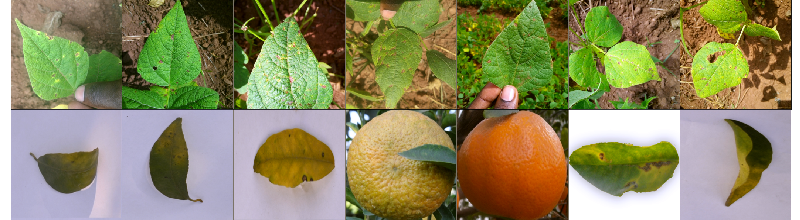
\includegraphics[width=0.8\textwidth]{imgs/citrus_beans_examples.png}
    \caption{Example images from the citrus and ibean data sets.
    The images in the top row are from ibean, and the bottom row is from the citrus data set.}
\end{figure}

The ibean dataset \citep{beansdata} contains 1296 images classified into three classes; Healthy, Angular Leaf Spot, and Bean Rust.
The data set provides a split for the images that will be the split that is used for the experiments.
The citrus leaves dataset \citep{citrusdata}, on the other hand, contains 759 examples of citrus fruits and leaves with six different classes; Black Spot, Canker, Greening, Scab, Melanose, and Healthy.
This set is quite tricky as it contains 609 images of leaves and only 150 images of actual citrus fruits, and some of the classes have very few images.
Some examples from the data sets are in Figure 6.1.
For the training split, the data will be split in 65/10/25 ratio for the training, validation, and test sets, respectively.
The goal of this kind of split is to have some relatively reliable test results by having proportionally larger than regular test set since there is so little data.
Both of these datasets have a relatively small amount of images available for training, so it should serve as a good basis for trying to train multi-task classifiers and give a glimpse into the adjustments that need to be made when training multi-task classifiers.
The goal for this experiment is to get familiar with the basics of how to create the multi-task models, and how to do the actual changes to the training loop in the Pytorch code to accommodate for the multi-task training.

When the two closely related datasets are used to train the model, we could expect the model to generalize better on both of them, as hopefully similar features would benefit both tasks.
But as the tasks are quite simple, the benefits can be relatively small as the likely accuracy for the single-task models should be quite high.
In the case of the citrus data set, learning to classify the citrus fruits could prove quite difficult, and for that, the bean leaves likely won't be of much help.
This model is depicted in figure 6.2.

\begin{figure}[h!] 
\centering 
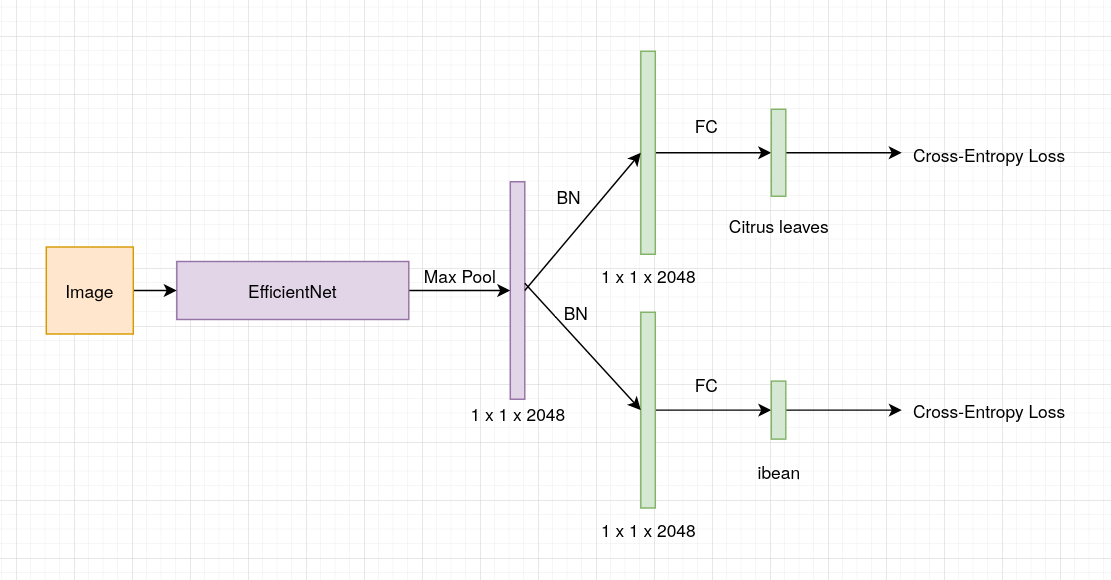
\includegraphics[width=0.8\textwidth]{imgs/object_classification_architecture.png}
\caption{Network architecture for two image classification tasks.}
\end{figure}

To further extend the generalizability, we will try to add a third somewhat similar classification task using the Oxford flowers102 dataset \citep{flowers102}, which contains 102 different types of flowers for classification. 
The assumption here would be that flowers could require similar features as the previous leaf classification tasks, thus when increasing the training data with a closely related task, we could increase the generalizability even further.

Multi-task and single-task models were created and evaluated for both EfficientNet and ResNet backbones.
For the single-task performance, in this case, the ResNet model did slightly better on both of the tasks achieving 96\% test accuracy on the beans dataset and 88\% test accuracy on the citrus dataset, and the EfficientNet model achieved 94\% and 84\% test accuracies on the tasks.
In terms of training, the most significant parameter is the sampling ratio of the two tasks.

The sampling was done with a random number to pick which data loader would be used for the current batch.
If the sampling is done by going through each of the datasets entirely one at a time, the model ends up at a point where only one of the tasks has good accuracy.
If the ratio is left as proportional to the data set size, the multi-task model ends up only learning to classify the ibean data set, and the accuracy for the citrus data will stay low.
After some experimentation, the suitable probabilities for achieving good results with the EfficientNet multi-task classifier were 0.66 for the citrus and 0.33 for the ibean data.
Interestingly, the same ratio does not directly transfer to the ResNet model. 
When we used the same ratio as with the EfficientNet, the model still seems to converge only on a good result for the ibean data set.
For the final results with the ResNet classifier, the sampling probability for the citrus dataset needed to be raised, and the value we ended up getting the best results with was 0.73.

\begin{table}[]
    \centering
    \begin{tabular}{lccl}
        \multicolumn{1}{l}{\textbf{}}    & \multicolumn{1}{l}{\textbf{ibeans}} & \multicolumn{1}{l}{\textbf{citrus}} & \multicolumn{1}{l}{\textbf{flowers}} \\ \cline{2-4}
        \textbf{Single-task models}      & \multicolumn{1}{l}{}                & \multicolumn{1}{l}{}                & \multicolumn{1}{c}{-}                \\ \hline
        \multicolumn{1}{l}{EfficientNet} & \multicolumn{1}{c}{94\%}            & \multicolumn{1}{c}{-}               & \multicolumn{1}{c}{-}                \\ \hline
        \multicolumn{1}{l}{EfficientNet} & \multicolumn{1}{c}{-}               & \multicolumn{1}{c}{84\%}            & \multicolumn{1}{c}{-}                \\ \hline
        \multicolumn{1}{l}{EfficientNet} & \multicolumn{1}{c}{-}               & \multicolumn{1}{c}{-}               & \multicolumn{1}{c}{97\%}             \\ \hline
        \multicolumn{1}{l}{ResNet}       & \multicolumn{1}{c}{96\%}            & \multicolumn{1}{c}{-}               & \multicolumn{1}{c}{-}                \\ \hline
        \multicolumn{1}{l}{ResNet}       & \multicolumn{1}{c}{-}               & \multicolumn{1}{c}{86\%}            & \multicolumn{1}{c}{-}                \\ \hline
        \multicolumn{1}{l}{ResNet}       & \multicolumn{1}{c}{-}               & \multicolumn{1}{c}{-}               & \multicolumn{1}{c}{97\%}             \\ \hline
        \textbf{Multi-task models}       & \multicolumn{1}{l}{}                & \multicolumn{1}{l}{}                & \multicolumn{1}{c}{-}                \\ \hline
        \multicolumn{1}{l}{EfficientNet} & \multicolumn{1}{c}{94\%}            & \multicolumn{1}{c}{88\%}            & \multicolumn{1}{c}{-}                \\ \hline
        \multicolumn{1}{l}{ResNet}       & \multicolumn{1}{c}{96\%}            & \multicolumn{1}{c}{89\%}            & \multicolumn{1}{c}{-}                \\ \hline
        \multicolumn{1}{l}{ResNet}       & \multicolumn{1}{c}{96\%}            & \multicolumn{1}{c}{91\%}            & \multicolumn{1}{c}{97\%}             \\ \hline
        \multicolumn{1}{l}{ResNet}       & \multicolumn{1}{c}{96\%}            & \multicolumn{1}{c}{-}               & \multicolumn{1}{c}{97\%}             \\ \hline
        \multicolumn{1}{l}{ResNet}       & \multicolumn{1}{c}{-}               & \multicolumn{1}{c}{85\%}            & \multicolumn{1}{c}{95\%}             \\ \hline
    \end{tabular}
    \caption{Accuracies on the data sets for both single-task and multi-task models with ResNet and EfficientNet.}
\end{table}

Training both tasks in a multi-task setting, we found that the accuracy on the citrus data set was increased, and ibean accuracy stayed the same.
Specifically, the accuracy for the EfficientNet classifier went up to 88\% and for ResNet up to 89\%.
The final model evaluated on the test set was the model with the highest average validation accuracy over the two tasks when trained for 25 epochs.
All the results are displayed in table 6.1.
The results show that even though these tasks were relatively simple and the accuracies for the single-task models were high, there was a benefit to be gained from multi-task training.
Here we mainly focused on getting good results on a fully shared backbone, and more experiments could be done by having fewer parameters shared between the tasks.
As an introduction to multi-task learning, the experiments show that picking the correct sampling ratio is extremely important for achieving desired results.
In that way, the sampling ratio seems quite unlike learning rate in that picking too small learning rate may lead to slow convergence but will most likely produce results in the end.
With the sampling ratio, it seems that the correct value needs to be found by experimentation, as a too low ratio for the citrus data gives accuracies that can be as low as 60\%.

Based on the results from the multi-task results on two tasks, we tried to add the third flower recognition task.
The flower recognition task has about 10 000 images and 102 classes, whereas the other two tasks have significantly less data and fewer classes.
On the two task experiment, it seemed that the sampling ratio should be relative to the task difficulty.
Here it would seem that the 102 class flower recognition should be much more difficult than the other two tasks, and we tried using sampling ratios in the range of about 0.5 to 0.7 for the flower task.
The best result achieved with these ratios was multiple percentage points below the single-task performance on all tasks.
However, when the flower task ratio was 0.1, it was possible to surpass the single-task results on all the tasks.
This training approach took significantly longer to converge to results.
The original sampling ratios converged in about five epochs to the best model, and the low flower ratio took about 50 epochs.
I started the training using the sampling ratio of 0.1 and decided to increase it up to 0.2 by the end of the training process.

When the training the model using the lower flower sampling ratio, it quickly converges close to the single-task performance on the two smaller tasks and slowly learns the flower task.
It is hard to say exactly why such low sampling ratios seemed to work.
Perhaps it has something to do with the difficulty of overfitting on a single task in a multi-task setting even though the small training set is seen so many times.
So the features for the smaller data sets are not just memorizing the pixels of the training set, but rather the features that generalize well.
Since the model already has good features for the smaller tasks and it is forced to find only a relatively minor shift in the parameters to learn the flower classification.
And seeing as the other tasks are improved as well, it shows that some of the features of the flower data are useful in the easier tasks.

From the three task models, the final model was picked as the one having the best average validation accuracy on all the tasks.
The final model wasn't just this model directly, though.
To get the final model, we froze all the shared weights and then did fine-tuning similar to what one might do when training a transfer learning classifier.
Having the model train on all the tasks using the frozen representations seemed to be useful.
The fine-tuning may be a good idea since, while training, the shared features are constantly shifting, and when one task is trained, it shifts the weights according to its gradients.
The other tasks won't have adjusted to the new, slightly shifted shared weights, which can lead to incorrect classifications.
When the shared weights are frozen, each of the task heads gets to learn the exact mapping from the shared representation to the outputs without them shifting during training.

All in all, these experiments validated the assumptions made about the multi-task training quite well.
Still, finding the sampling ratio is very laborious and not very intuitive.
This is why the results for the citrus and flower pair are worse since we spent less time finding the optimal ratios and mainly verified that it roughly works as expected.
Perhaps it could be automated to get somewhat decent indications of what should be tried.
The problem, in the end, is that even if some kind of grid search could be applied, it would take very long to predict the final metrics of the models, and as seen in the discrepancy of the flower ratios, it could take many epochs to get the final results.
Perhaps some kind of dynamic sampling ratio, where the task lowest relative to the expected accuracy is sampled more, could be beneficial.

\section{Multi-label classification}
For multi-label prediction, there can exist a problem where not all classes are restricted to only their data sets.
For example, a photo of a dog taken outdoors can contain other classes such as a person, sky, or sea.
These may not be labeled for that set but could be classes of interest.
If we train models on incorrect labels, it can lead to unlearning as the model may make correct predictions but is punished due to the absence of the labels for the images.
However, if the problem is posed as a multi-task binary classification problem over several classes, each task can have its own distinct data set with labels for only the single task.
Then upon training on an image containing other classes, there is no inverse learning as the image will not try to learn the other classes if there exists no certainty of that label.
Still, the problem is not gone as often any dataset has at least some mislabeled examples.

\begin{figure}[h!] 
\centering 
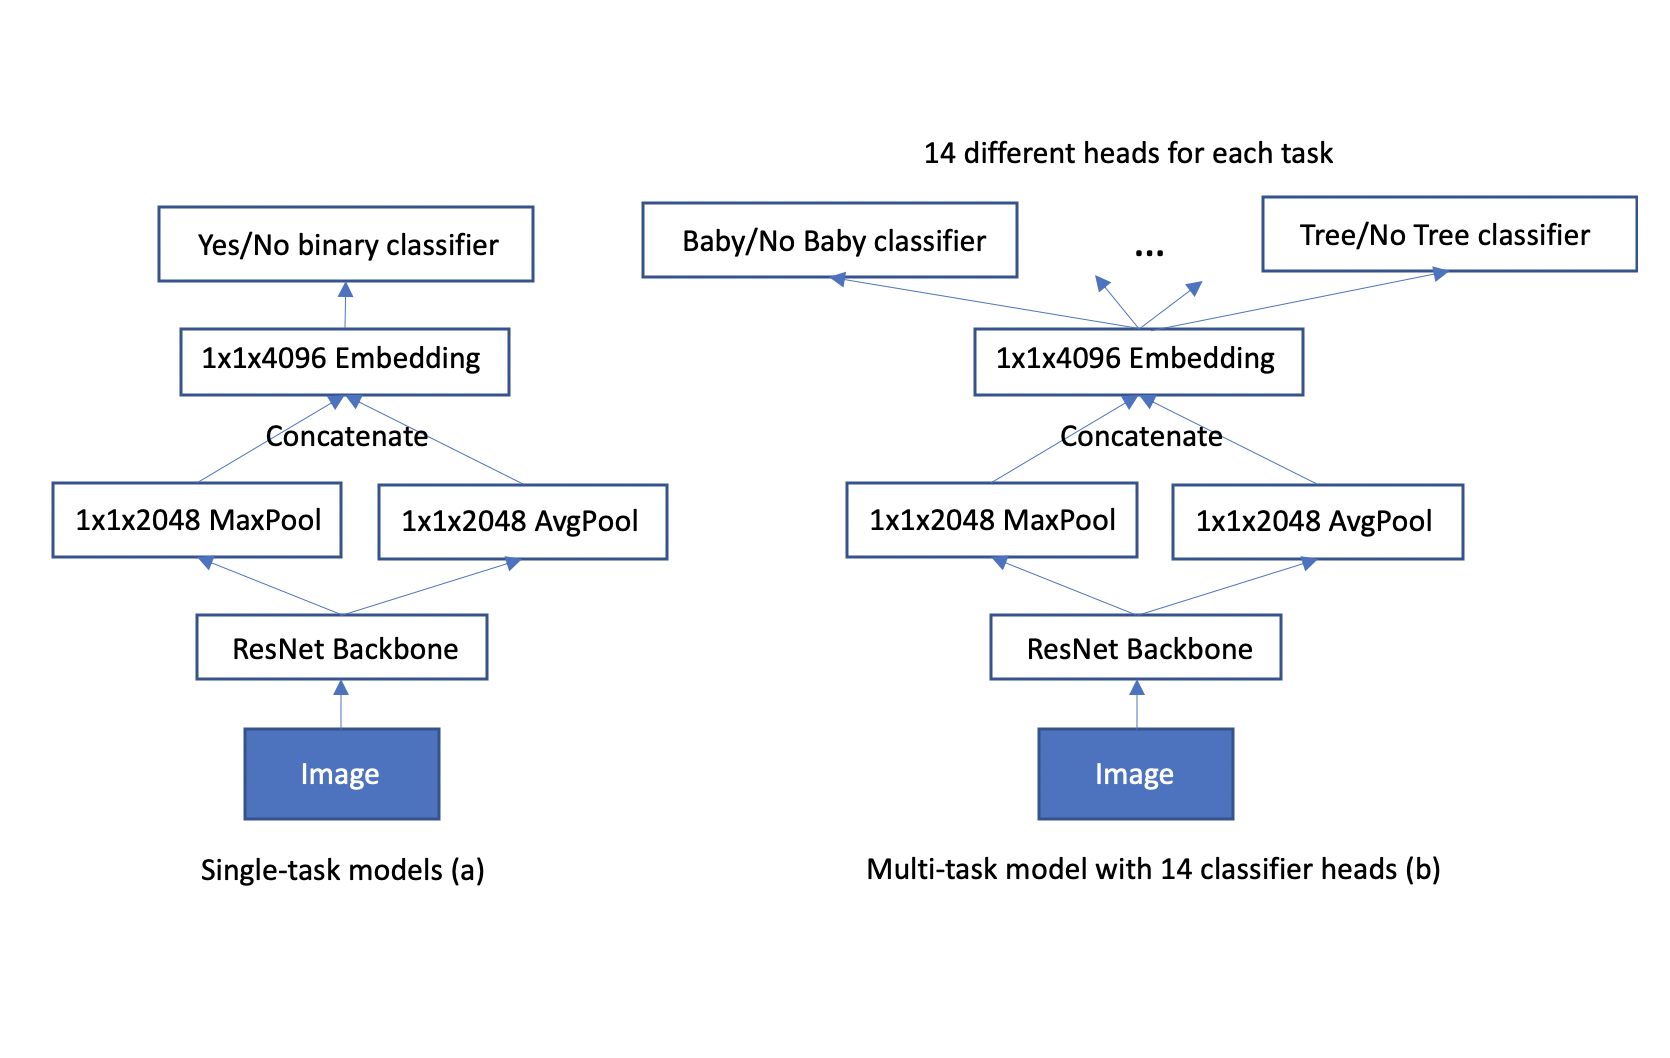
\includegraphics[width=0.8\textwidth]{imgs/image-labeling.png}
\caption{Architectures for both single-and multi-task models. The model (a) is the single-task model, which is the same for all 14 tasks. Model (b) is the Multi-task model, which contains 14 heads for each of the classification tasks. For these classifiers we took both max and average pool to create the embedding.}
\end{figure}

We will run some experiments on a 14 class multi-label prediction with some overlap between the classes in the images.
The 14 head multi-task model structure and the structure of the 14 identical single-task models are shown in Figure 6.3.
The goal here would be to see how what kind of a difference there would be in training with a single-task and multi-task model over all of the labels.

\begin{table}[]
    \centering
    \begin{tabular}{lccl}
        \multicolumn{1}{l}{\textbf{}}    & \multicolumn{1}{l}{\textbf{Multi-task}} & \multicolumn{1}{l}{\textbf{Single-task}} \\ \cline{2-3}
        \multicolumn{1}{l}{People} & \multicolumn{1}{c}{90\%}            & \multicolumn{1}{c}{89\%}                           \\ \hline
        \multicolumn{1}{l}{Man} & \multicolumn{1}{c}{87\%}               & \multicolumn{1}{c}{84\%}                        \\ \hline
        \multicolumn{1}{l}{Woman} & \multicolumn{1}{c}{86\%}               & \multicolumn{1}{c}{87\%}                           \\ \hline
        \multicolumn{1}{l}{Baby}       & \multicolumn{1}{c}{87\%}            & \multicolumn{1}{c}{93\%}                           \\ \hline
        \multicolumn{1}{l}{Sea}       & \multicolumn{1}{c}{89\%}               & \multicolumn{1}{c}{96\%}                        \\ \hline
        \multicolumn{1}{l}{River}       & \multicolumn{1}{c}{89\%}               & \multicolumn{1}{c}{88\%}                           \\ \hline
        \multicolumn{1}{l}{Bird} & \multicolumn{1}{c}{88\%}            & \multicolumn{1}{c}{89\%}                        \\ \hline
        \multicolumn{1}{l}{Car}       & \multicolumn{1}{c}{85\%}            & \multicolumn{1}{c}{94\%}                        \\ \hline
        \multicolumn{1}{l}{Clouds}       & \multicolumn{1}{c}{93\%}            & \multicolumn{1}{c}{93\%}                        \\ \hline
        \multicolumn{1}{l}{Dog}       & \multicolumn{1}{c}{87\%}            & \multicolumn{1}{c}{93\%}                           \\ \hline
        \multicolumn{1}{l}{Flower} & \multicolumn{1}{c}{85\%}            & \multicolumn{1}{c}{93\%}                        \\ \hline
        \multicolumn{1}{l}{Night}       & \multicolumn{1}{c}{87\%}            & \multicolumn{1}{c}{92\%}                        \\ \hline
        \multicolumn{1}{l}{Portrait}       & \multicolumn{1}{c}{89\%}            & \multicolumn{1}{c}{91\%}                        \\ \hline
        \multicolumn{1}{l}{Tree}       & \multicolumn{1}{c}{87\%}            & \multicolumn{1}{c}{92\%}                           \\ \hline
        \multicolumn{1}{l}{Average}       & \multicolumn{1}{c}{88\%}               & \multicolumn{1}{c}{91\%}                        \\ \hline
    \end{tabular}
    \caption{Accuracies on the data sets for both single-task and multi-task models. 
    The accuracy is the proportion for correct labelings in the balance evaluation set, so pure guess would result in 50\% accuracy.}
\end{table}

The dataset is a collection of 15000 images that have labels for some of the classes.
The number of labels for each task is highly varied.
The smallest tasks have dozens of images, whereas the largest ones have thousands.
From this dataset, we will take for each class a 15\% cut for validating the performance.
In this case, we will pose our main problem as a binary classification problem.
For each of the tasks, we will train a classifier telling if the label exists in the image or not.
The classifier will use a ResNet-101 as a backbone, and the head will be a regular fully connected layer connected to a positive and negative class for each of the tasks.
For the single-task models, we will have the same ResNet backbone as for the multi-task model.
The main metric that we will compare will be the ratio of correct labelings per class.
Since we pose this as a binary classification task, it is easy to guarantee that our test sets have an exact 50/50 split for positive and negative classes.
Similarly, while training, we can oversample the positive classes in a way to guarantee that each batch will have half positive and half negative classes.
This way, we won't learn classifiers that are biased toward predicting the absence of the label due to the small number of images for that class.
The control over the sampling of the data is a very beneficial trait of the multi-task problem setting.

To train the multi-task model, we experimented on various sampling ratios to find the best model.
Manually giving a meaningful sampling ratio is quite difficult due to the relatively large number of tasks in this multi-task model.
The various sampling ratios we tested for this data were equal sampling, data proportional sampling, and finally, some manual adjustments to the proportional sampling based on the results.
The proportional sampling was the one that produced the final best model.
It is quite an interesting result, considering just how small some of the classes are relative to the entire data set.
We tried adjusting the proportional ratios based on the difference from the single-task accuracies but could not find ratios that would have improved the performance.
Based on the previous results, we could say that there likely exists some ratios that could provide superior results, but finding them is too expensive.
With the best model, which was chosen based on the average accuracy on the validation data, the model achieved an average of 88\% accuracy in labeling all the tasks.
By average, we mean taking the accuracy of each task separately and averaging those averages and not the total ratio of correct classifications.

One new thing that we noticed when training on this data set was that with too high learning rates, the experiments were not very repeatable.
It seems that in a multi-task setting, it is not easy to tell that the learning rate is too high.
In this case, when the learning process seemed to progress in a manner that we would call expected, the learning rate might actually be too high.
With a slightly too high learning rate, it seemed like it is relatively random, whether the model reaches the best weights.
Most likely, the sampling ratios matter here quite a lot, but with the same sampling ratios and a slightly too high learning rate, there didn't seem to be a guarantee that anything close to the best model would be reached.
Maybe this has something to do with the large variance in the size of the datasets.
With more dynamic sampling ratios, the problems might solve themselves, as then some tasks would hopefully not get stuck at low accuracies.
We noticed here the same thing as in the leaves experiment that a long training process that slowly approaches the optimum seems to produce the best results in the end consistently.
Maybe this means that finding the intersection that can solve all the tasks optimally is relatively small and easy to overshoot with too large learning rates.
Similarly, with incorrect sampling ratios, the model would never be able to reach the weights needed for the shared optimal solution.
To deal with the imbalanced classes, we also tried to add an exponent to the loss like in the focal loss, though it is unsure if it was useful or not.
But in theory, it should allow for the network to learn more from the cases where it is unsure.
Also, it would be yet another parameter to tune, as it is hard to say what exactly the exponent should be for the best results.

The single-task model training was done similarly to the multi-task model and by using the same data loading techniques.
This way, we reached an average accuracy of 91\%, beating the multi-task model slightly.
All the task-specific results for both multi- and single-task models are collected in Table 6.2.
Some part of the errors is due to the misclassification of the data, based on a random sample, around 2\% of the labels are wrong.
These results yet again show that it is possible to learn different tasks using the same representations.
Yes, in this case, the multi-task accuracy didn't match the single-task counterparts, but they are relatively close.
And all this is not really a fair comparison as the single-task models account for a total of around 14 times as many parameters.
If the single-task models were trained on significantly smaller backbones, the multi-task model could be more accurate, showing the benefit of using larger models over multiple tasks.
And even picking the smallest ResNets, the number of parameters over 14 tasks would be larger than a single ResNet101.

\section{Object detection and image classification}
In this section, we will use multiple data sources and combine them into a single powerful object detector.
To be specific, our goal is to create an object detector for 37 different cat and dog species.
The two datasets that we will use are the COCO dataset \citep{COCO} from which we will take the cat and dog classes and the Oxford-IIT Pet Dataset \citep{catsdogs}, which comprises of images with labels for the 37 different cat and dog species that we will detect.
In these experiments, the backbone used will be EfficientNet-0, which will be used in the EfficientDet architecture as well as an independent EfficientNet backbone.
The base for the code of the detector uses this Pytorch implementation of EfficientDet \citep{pytorch-efficientdet}.
The base model is then modified to meet the needs of our experiments.

There are multiple ways to approach this problem.
We will train two different models to see how the results differ.
The first approach is to do a brute-force two-stage detector, where we share the common backbone.
In this approach, the detector would try to learn to detect the dog and cat classes from the COCO dataset, while an object classifier is trained using the same backbone as the detector.
The object classifier is then responsible for giving the actual class of interest.
This way, the training is relatively simple, and the backbone would be used recursively.
Specifically, the detector would generate the regions for the animals that would be cropped and pushed through the backbone, this time to the classifier head.
This recursive use of the backbone is efficient in terms of the parameters, but running images through the same backbone twice could turn out to be too expensive as it would double the inference time.

\begin{figure}[h!] 
\centering 
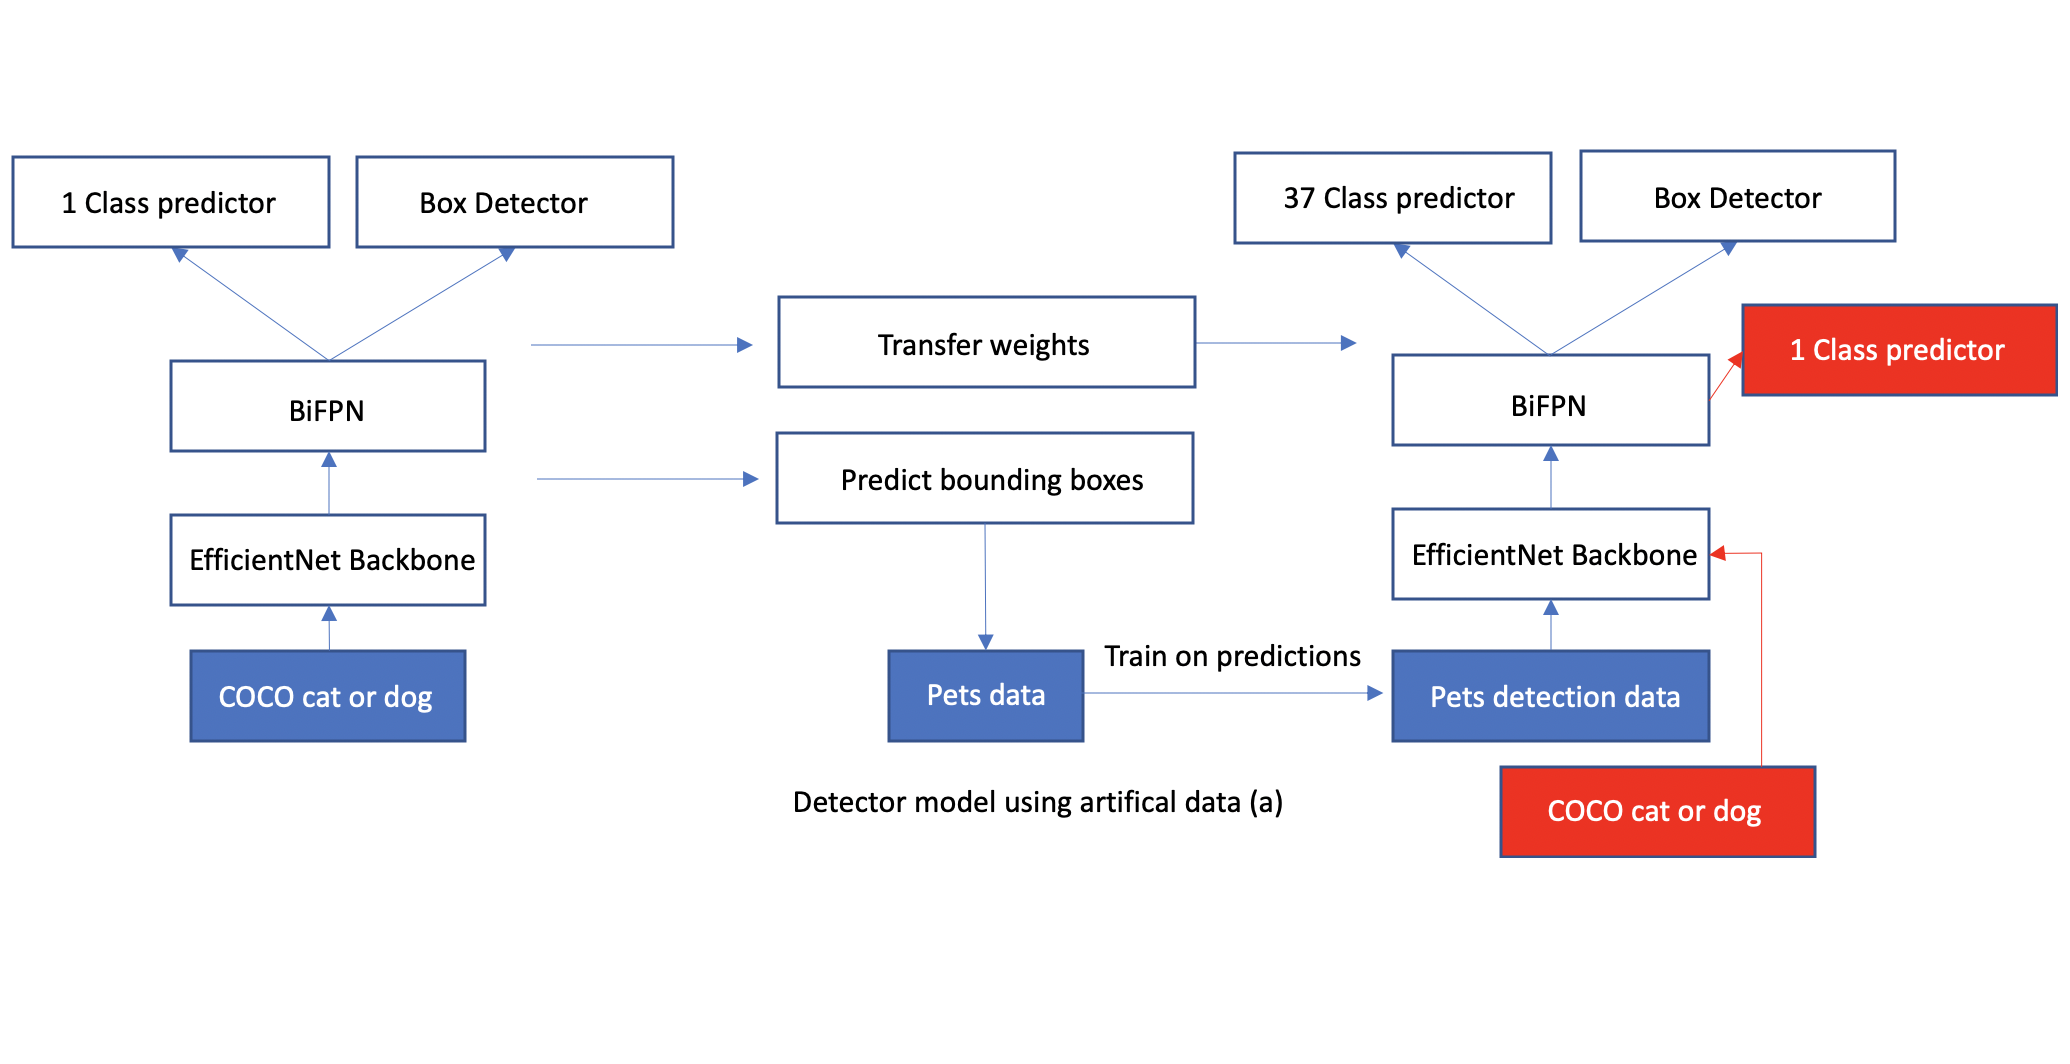
\includegraphics[width=0.8\textwidth]{imgs/object_detect_combine.png}
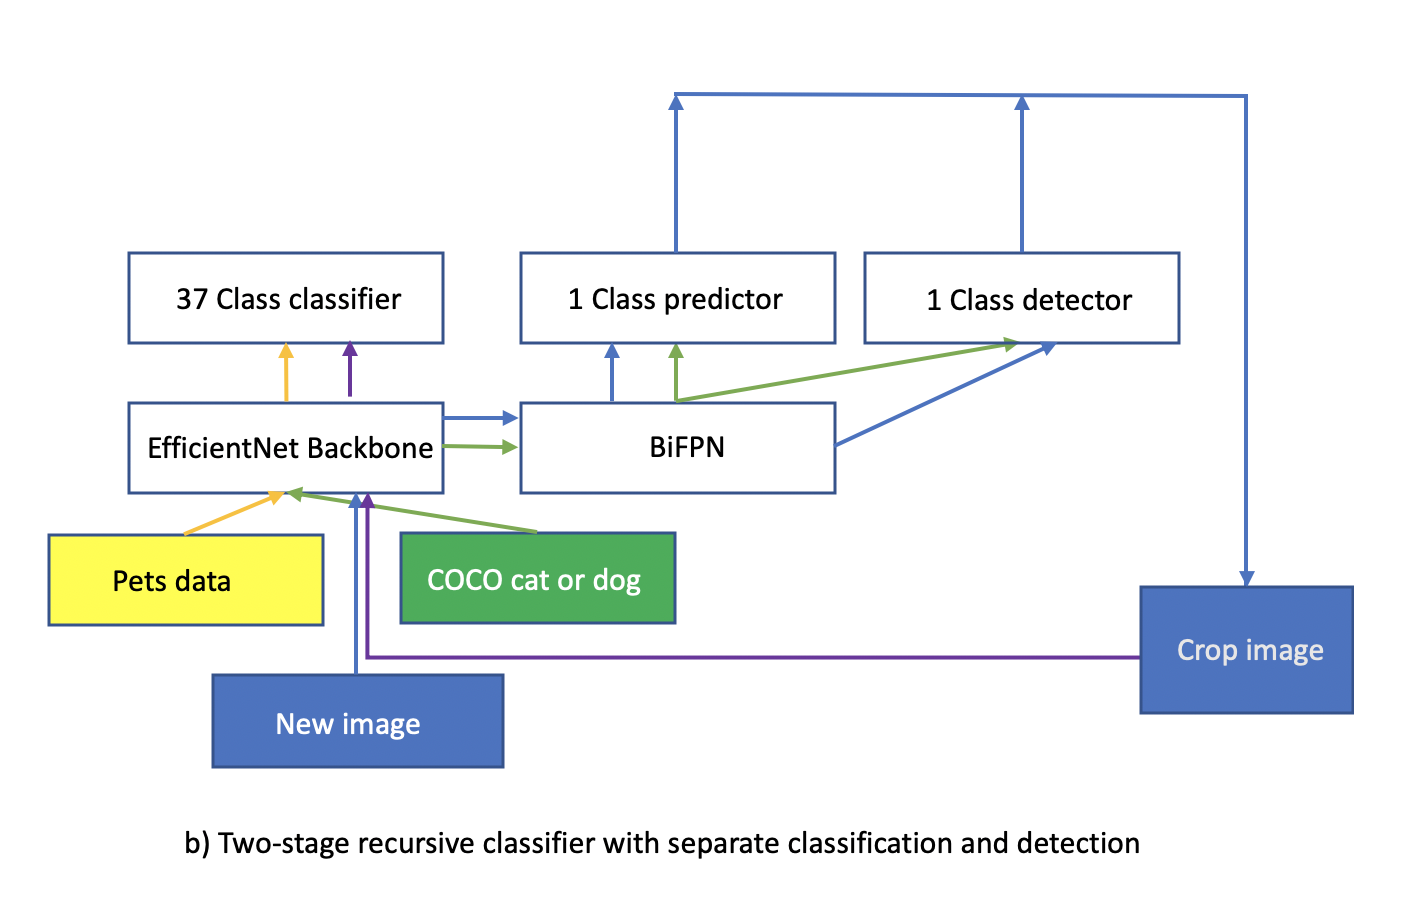
\includegraphics[width=0.8\textwidth]{imgs/recursive.png}
\caption{EfficientDet models for solving the object detection problem. In a), we have the basic object detector. We show how we train on the COCO data first and then transfer the weights to the model for the pets data with predicted bounding boxes. In red the additions needed to train on both the original data and artificially labeled are shown. Both tasks could share the weights for the detector but would need to have their own class head.  In b), we have the recursive object detector. In yellow, we describe the path to train on the pets data. With green, we describe the path to train the cat or dog object detector. In blue, we show the first cycle of a new prediction. With purple, we show the second cycle for the new detection.}
\end{figure}

The second way of approaching this problem is to first train a model on the COCO classes and to create a detector for the cat and dog classes.
Using the high-level model, we can automatically create acceptable object detection labels for the 37 classes in the pets dataset.
Then we can initialize a 37 class object detector using the weights of the two-class model.
By having such a well-initialized model for the detection, the second part of the training focuses on learning the features to differentiate between the very similar classes.
An interesting question here is just how well the object detector works when the classes are so similar.
In an image classifier setting, it would make sense that the model could learn the subtle features that are unique to each of the classes.
As we previously covered, the object detector is a multi-task problem. 
It follows that the network has to both decide the anchors most likely containing an object and also determining the class of the object.
If we look at the classes for the COCO dataset for object detection, for example, we can see that there are 80 classes, but they are relatively difficult to mix up due to being quite distinct from one another. 
In Figure 6.5, we have an example of two images from the pets dataset showing two classes that would be relatively easy to mix up.

\begin{figure}[h!] 
\centering 
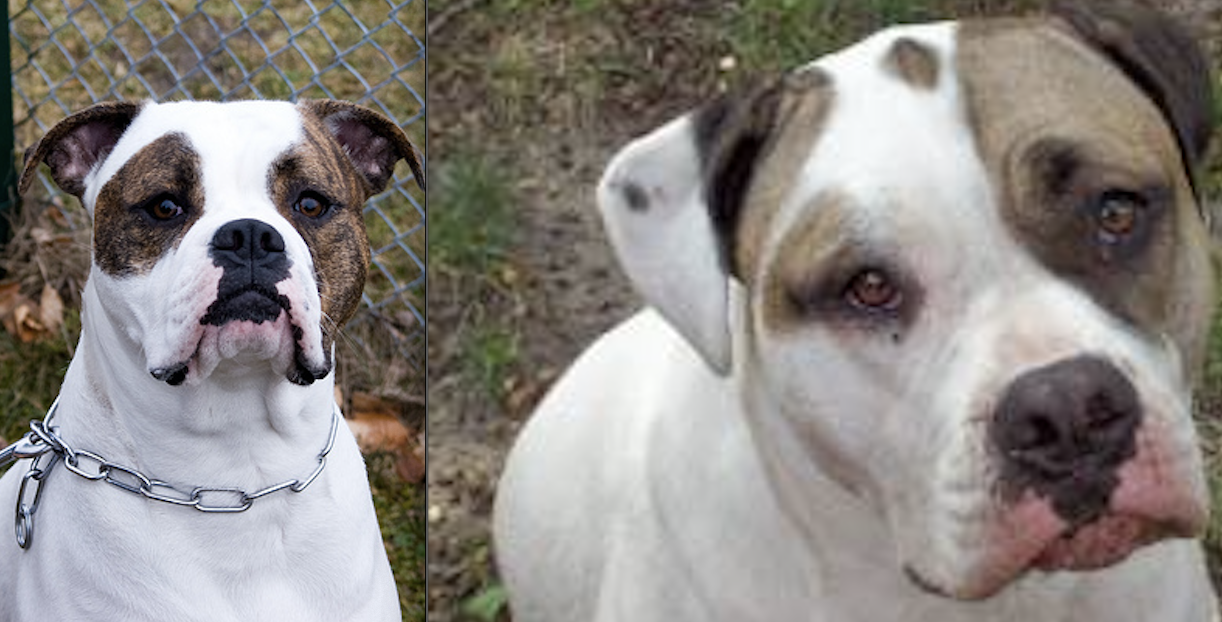
\includegraphics[width=0.8\textwidth]{imgs/pets-example.png}
\caption{Example of two very similar classes in the pets dataset. On the left is an American bulldog and on the right is an American pit bull terrier.}
\end{figure}

To evaluate the effects of both approaches, we will look at multiple metrics.
Since the two approaches are quite different, we can't make an entirely fair direct comparison between them.
To get somewhat of an idea for how well the models detect our 37 different classes, we will use a slightly arbitrary metric.
We will measure the accuracy of the detector on our test set for the pets dataset.
A positive example is one where the detector gives the highest confidence to the correct class.
This is a somewhat simplified version of measuring the detector performance.
The baseline scores for our EfficientNet-0 model are 92\% accuracy on the pets dataset and a 0.55 AP on detecting the cat and dog classes in the COCO dataset.
We will calculate these same scores for the recursive model to see how close the multi-task model can get.
To compare the two approaches, we will calculate the accuracy of correctly detected species in a set of the pets dataset.
The labels are not going to be perfect as they are generated by the model automatically, but should show if there are major discrepancies in the performance between the two approaches.

To train the single-stage model, we first created a new dataset in the COCO format from the dog and cat classes.
Instead of having two classes, we combined both dog and cat into a single category as the goal is to detect them as well as possible, and we are not interested in identifying whether it is a dog or a cat.
It is important to set the category id to be one instead of zero when training the object detector when there is only one class since otherwise, there will not be any predictions for the background.
With this new dataset, we initialized the EfficientDet model and trained it to detect the single class from the COCO dataset.
We first fine-tuned the head for ten epochs and then fine-tuned the entire network for 40 more epochs, and we picked the model with the lowest validation loss as the best one.
The chosen model achieved 0.54 AP when tested.
Then we created a new COCO style dataset out of the pets dataset.
To get the annotations, we ran the images through our one-class object detector and labeled all found boxes with the class of the image from the pets dataset.
The COCO format requires the labels as a tuple of four numbers signifying the x and y coordinates of the top left of the bounding box, followed by the bounding box width and the height.
Since most of the images in the pets dataset contain only a single animal, we could tell that there were incorrect boxes as the number of annotations was about 10-15\% higher than the number of images.
The bounding boxes were most likely not perfect, but good enough to get decent results.
We initialized the model with the weights of the original object detector, which meant that the regression loss for the model was consistently low.
So the training mostly focused on learning to minimize the classification loss with the new 37 classes.
Since this was a much more difficult problem than the original, it took a bit longer to reach the best model.
Evaluating the model on the artificial labels of the validation set gave an AP score of 0.55.

There are a few ways this kind of training could be extended to possibly get even better results.
We could attempt to train the largest possible model to get the best possible results on the original dataset so that the artificial labels for the unlabeled dataset would be the best possible.
We could create two heads in the object detector to train the detector on both the original COCO images and the new images in a multi-task setting to hopefully get a more general detector.
The training could get better if multiple cycles were completed, and the training would work in a semi-supervised way.
So what we used here would be the first labels for the new dataset.
The training would be done jointly on both datasets, as previously proposed.
Every n epochs, we would generate new bounding boxes for the pets dataset, to finally reach the optimal bounding boxes for the classes in the pets dataset.
Finally, we could do the label transfer also in the other direction.
Since the COCO has the correct bounding boxes, we could run the image classifier trained on the pets dataset on those boxes to generate the actual animal species for them.

The recursive model heavily relies on sharing the EfficientNet backbone in the detector between the classifier head and the detector head.
The model is recursive because, on the first pass, we will find the cat or dog regions from the model using the detector head.
Thus, the detector head is predicting only a single class as the distinction between the cat or dog class is of no interest in the detector.
Given these detected objects, we can crop them from the original image and pass through the other head, which is concerned with classifying the image into the 37 classes of interest.

For the recursive two-phase model, we trained it in a very similar fashion to the previous multi-task models.
In this case, we ran the experiment with only a few sampling ratios, of which a 50/50 split produced the best results.
The object detector only required adding the final classification head on top of the backbone, and then the model could be trained with a basic multi-task training loop since the EfficientNet backbone that we wanted to use is already a part of the EfficientDet model.


\begin{table}[]
    \centering
    \begin{tabular}{lccl}
        \multicolumn{1}{l}{\textbf{Pets classification}}    & \multicolumn{1}{l}{\textbf{}}  \\ \cline{1-2}
        \multicolumn{1}{l}{EfficientNet-B0 baseline} & \multicolumn{1}{c}{93\%}                    \\ \hline
        \multicolumn{1}{l}{Recursive detector task head}       & \multicolumn{1}{c}{89\%}                       \\ \hline
        \\
    \end{tabular}
    \caption{
    This table lists the accuracy for pets classification without localisation based on the baseline model and the classifier head in the recursive model.
    }
\end{table}


\begin{table}
    \centering
    \begin{tabular}{lccl}
        \multicolumn{1}{l}{\textbf{Cat or dog detection}}    & \multicolumn{1}{l}{\textbf{}}  \\ \cline{1-2}
        \multicolumn{1}{l}{EfficientDet-D0 baseline} & \multicolumn{1}{c}{0.54}                       \\ \hline
        \multicolumn{1}{l}{Recursive detector}       & \multicolumn{1}{c}{0.52}                    \\ \hline
    \end{tabular}
    \caption {
        This contains the AP score for detecting the single cat or dog class for the baseline and the recursive detector.    
    }
\end{table}
\begin{table}
    \centering
    \begin{tabular}{lccl}
        \multicolumn{1}{l}{\textbf{Custom pets detection metric}}    & \multicolumn{1}{l}{\textbf{}}  \\ \cline{1-2}
        \multicolumn{1}{l}{EfficientDet-D0 trained with artificial data} & \multicolumn{1}{c}{85\%}     \\ \hline 
        \multicolumn{1}{l}{Recursive detector with separate heads}       & \multicolumn{1}{c}{91\%}                       \\ \hline
    \end{tabular}
    \caption {
        This table compares the EfficientDet trained on artificial data and the recursive model in detecting the 37 pets classes.
        Here the metric is the proportion of correct classifications in the most confidently detected box.
    }
\end{table}
\begin{table}
    \centering
    \begin{tabular}{lccl}
        \multicolumn{1}{l}{\textbf{37 class object detection}}    & \multicolumn{1}{l}{\textbf{}}  \\ \cline{1-2}
        \multicolumn{1}{l}{EfficientDet-D0 artificial data 37 classes AP} & \multicolumn{1}{c}{0.55}                       \\ \hline
    \end{tabular}
    \caption {
        The AP score on 37 class object detection for the model with artificial data.
    }
\end{table}

To compare the models, we have collected the various metrics in Tables 6.3 to 6.5, grouped by the comparable metrics. 
The pure object detector for 37 classes had a 0.55 AP score on the artificially labeled dataset of the pets, and this is mildly higher than the base AP for the cat or dog detector.
While the number seems impressive given the number of highly similar classes, it is not exactly comparable to the baseline due to the fact that the pets dataset is not that varied in terms of having many or different sized animals.
Furthermore, the bounding box labels are created by the initial state of the 37 object detector, which likely causes the accuracy for the bounding boxes is going to be very high.
The regression loss of localizing the boxes stays very low and stable throughout all of the training, showing that likely the detection part does not change that much.
In our artificial detection evaluation metric, this pure detector achieved an 85\% accuracy.
The accuracy is relatively high, given the difficulty of detecting and classifying such similar classes.

The recursive multi-task model reached again slightly lower accuracies than the single task counterparts.
The AP score on the cat or dog detection task dropped by 0.02, and the accuracy on the pets classification dropped by 4\% to 89\%.
Interestingly, the detector task had a higher accuracy than the classification head had on the pets test set.
The better accuracy could result from the fact that classifying a cropped animal is easier than to classify it within a larger frame.
And since the object detector is relatively decent at finding the cat or dog candidates as a combination, these achieve better results.

Based on the numbers, we could say that the two-stage detector seems to be the better one.
The main downside to doing the two-stage detection is the fact that it would have to work one frame behind the video.
Since on the first loop, we would detect our objects in the first frame.
On the second frame, we would pass the second frame and the cropped images that we found in the first frame.
If the classification is done in this manner, the inference time cost won't be that much as it will be just the head to get the classification outputs.
In the case that multiple videos would be run in parallel, this could possibly not be possible as at some point, the input could be too large to handle as a single batch.
On the other hand, the pure detector doesn't need such considerations.
The pure detector's problem is that it has some obvious downsides due to the artificial training set that was created for it.
Whereas the recursive model does relatively as well on all kinds of data, the pure detector seems to have issues when there are multiple objects to detect, or the size varies.
These issues likely stem from the fact that the pets dataset consists mostly of single relatively large animals, which is not always the case.
Because the training and test sets are from the same source, they are relatively similar, so the performance is very transferable between those tasks.
Some of the previously mentioned ways of training could alleviate this problem.
Perhaps by having two classifier heads and doing auxiliary training on the COCO cats and dogs could make the detector detect the animals better, and hopefully, the classifier could solve the problem for all sizes from the single source.
This modification is also pictured in Figure 6.4.

\section{Detection and segmentation with EfficientDet}
In the EfficientDet paper \citep{efficientDet}, the authors point out that it is relatively simple to use the same EfficientNet backbone and BiFPN neck to do image segmentation as well.
Here we will attempt to train such a model but in a multi-task setting.
Our goal is to use the Kitti \citep{kitti} road segmentation data set to train a segmentation model, and the COCO dataset to train an object detector.
Since they both should be trainable on the same backbone and neck, we will see how good of a multi-task model we can create by sharing the entire detector.

Since we have not talked about image segmentation, we will briefly cover what it is about.
Image segmentation is also a very popular and important task with applications in many domains.
The goal for an image segmentation model is to determine the meaning of an image on a per-pixel level.
For example, in our case, we are going to train a model on the road segmentation data where the goal is to predict where the current lane goes, so we would like to know where the pixels that represent the current lane the car is on are.
So the output is a mask telling what class each pixel in the image belongs to.
An example image and its segmentation mask are shown in Figure 6.6.

\begin{figure}[h!] 
\centering 
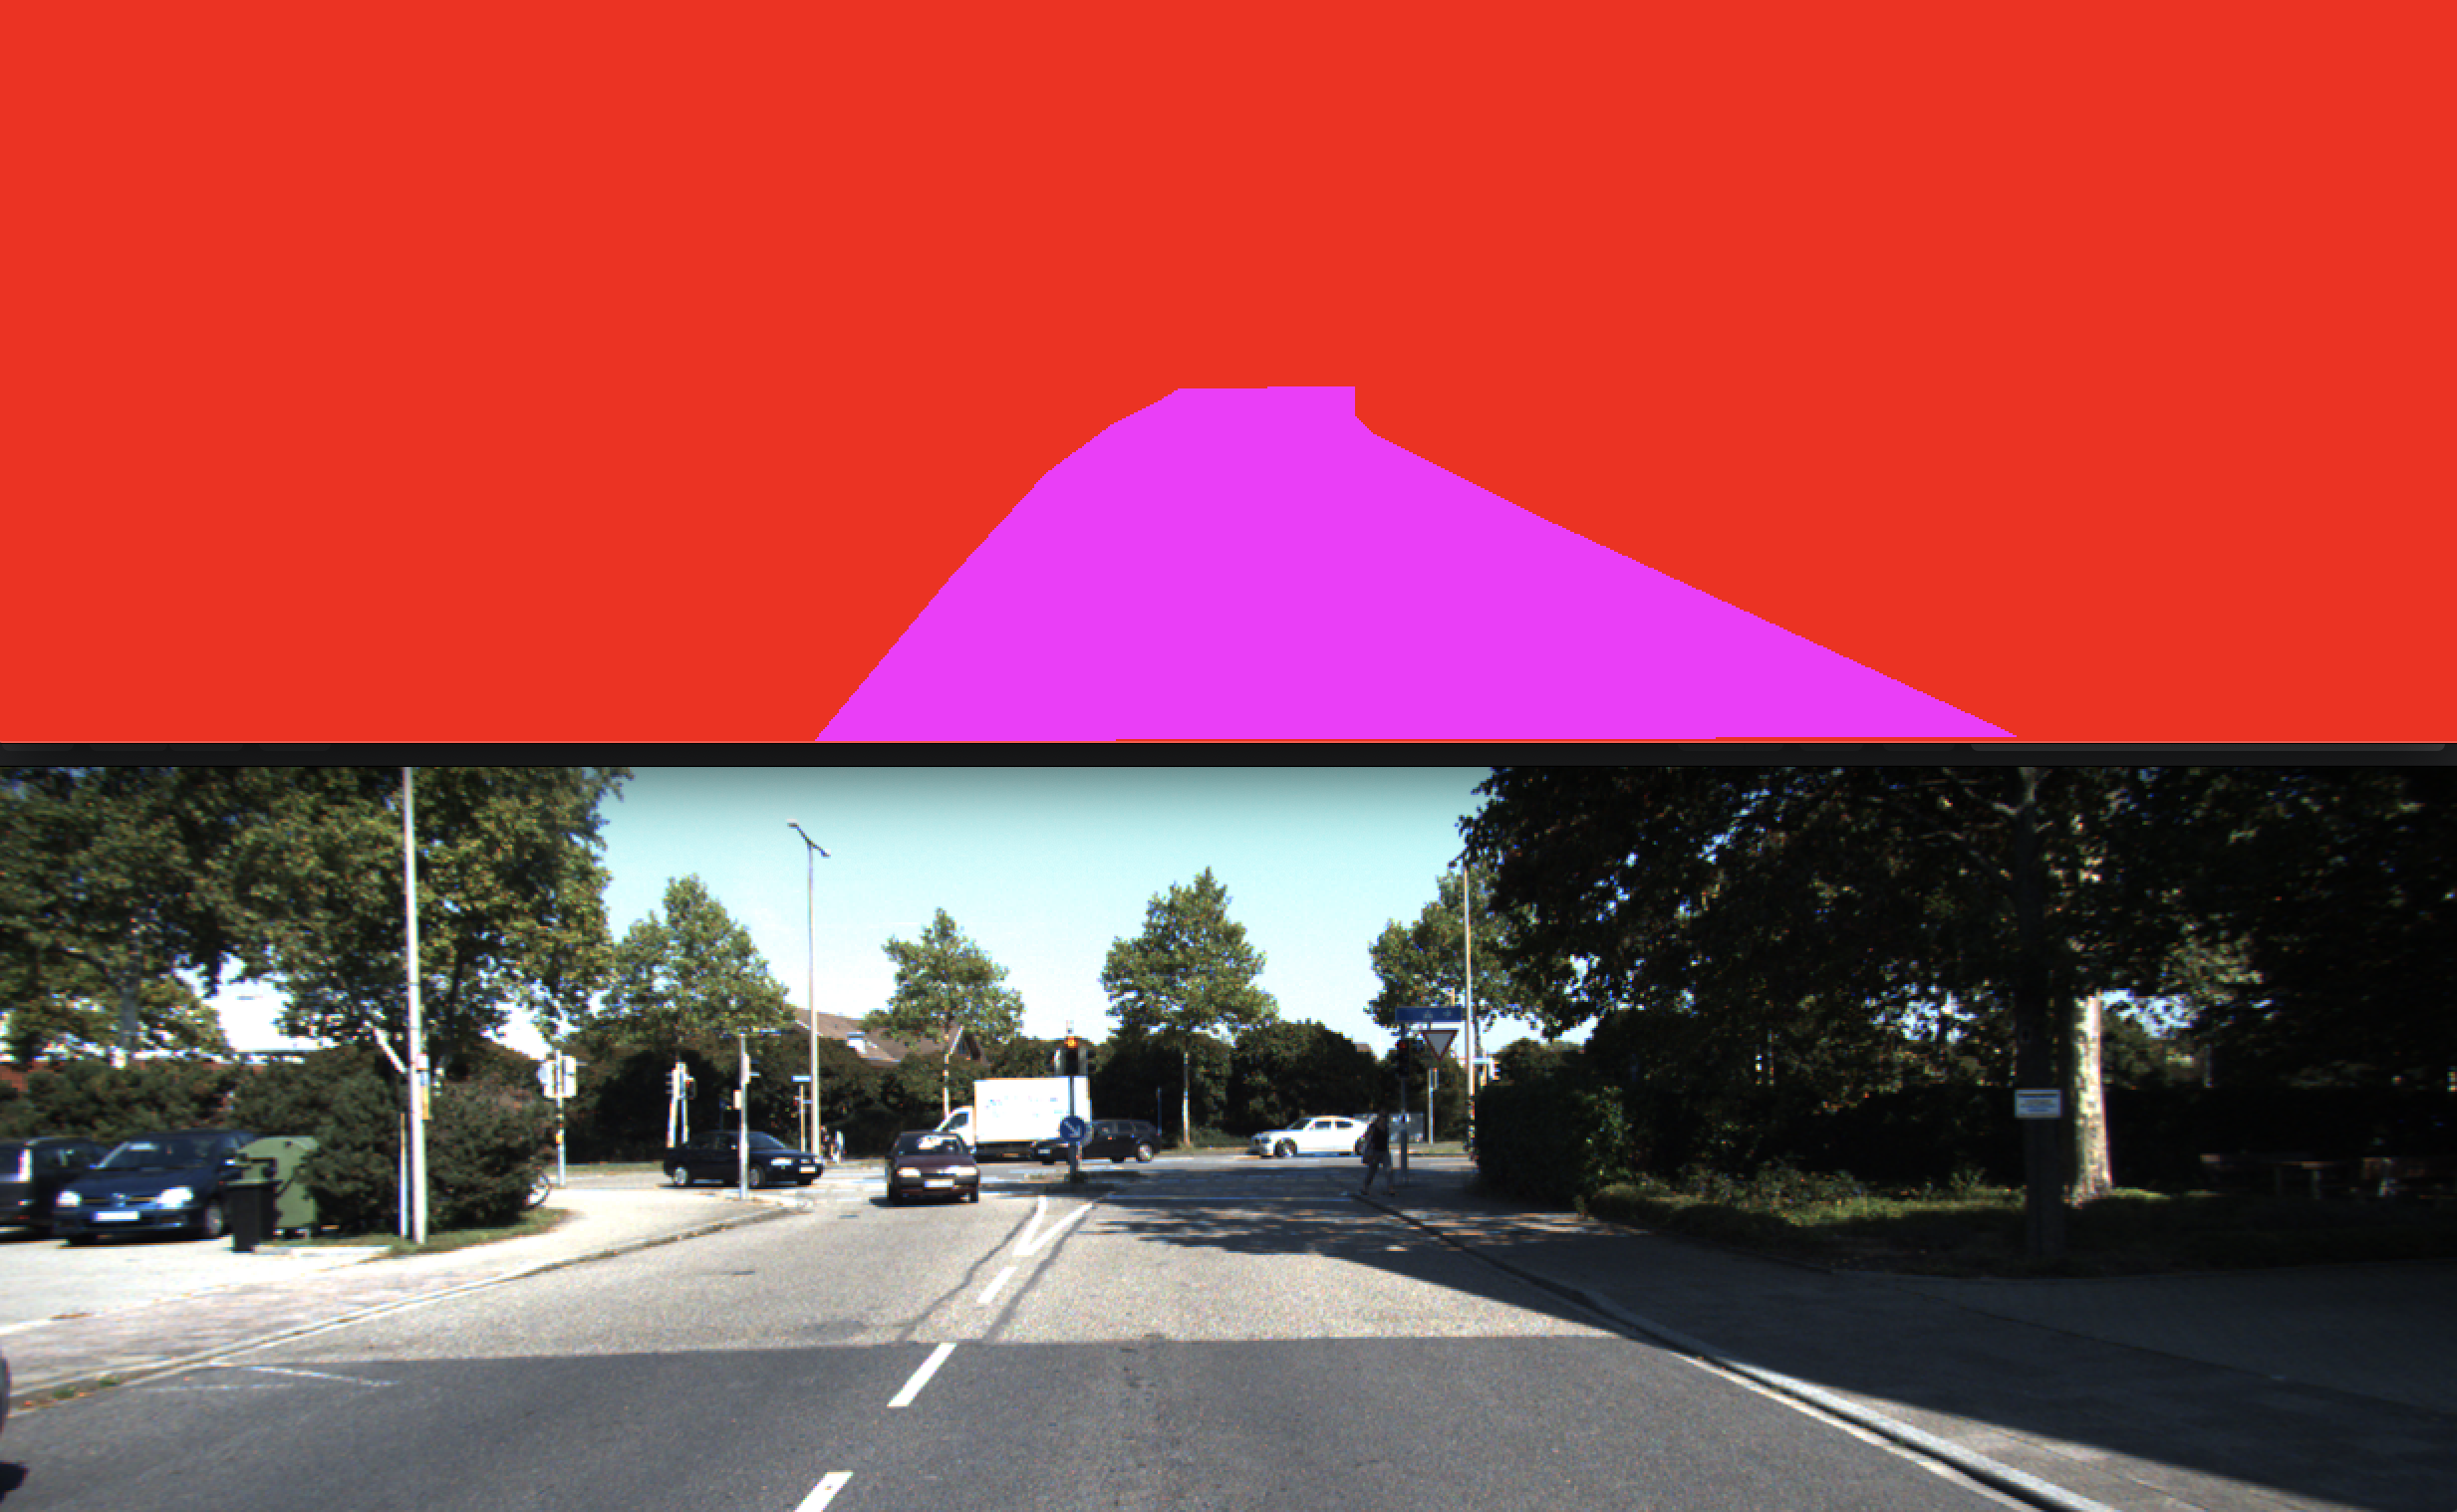
\includegraphics[width=0.8\textwidth]{imgs/segmentation-example.png}
\caption{An example of the annotations and an input image from the Kitti \citep{kitti} road segmentation data.}
\end{figure}

Here our goal is not to create a very accurate classifier but more to evaluate how difficult it is to take two very special problems and solve them by sharing as much as possible.
To create the model, we could use a U-Net \citep{unet}, which is an architecture specially designed for image segmentation.
We could adapt the U-Net architecture to EfficientNet and easily fit it with our backbone.
However, by using the EfficientDet, we get a chance to share more, and it is a much more advanced way of doing image segmentation, producing better results \citep{efficientDet}.

There is no complete implementation of the EfficientDet image segmentation head, and the authors don't really describe it too much in the paper.
To create the model, we took the EfficientDet detector as a base and augmented it with a segmentation head.
The segmentation head was based on the implementations of BiFPN segmentation from \citep{segment_pytorch}.
After creating multiple multi-task models, the creation and modification of the training loop were no longer so difficult to adjust to the new task.
Figuring out exactly how to add the new task into the existing model architecture took a while to find the exact values that the segmentation model needs for creating outputs.
After configuring data loaders and the model, the training was pretty much along the lines of the previous models we have covered.
The results for our models were along the lines that we have seen previously, the multi-task model being a few points below the single-task models.
It could be possible here that the segmentation model could get better if it had its own BiFPN network and could only share the backbone with the detector, but we did not have enough time to run all possible experiments.
Our modified EfficientDet architecture is shown in Figure 6.7.

\begin{figure}[h!] 
    \centering 
    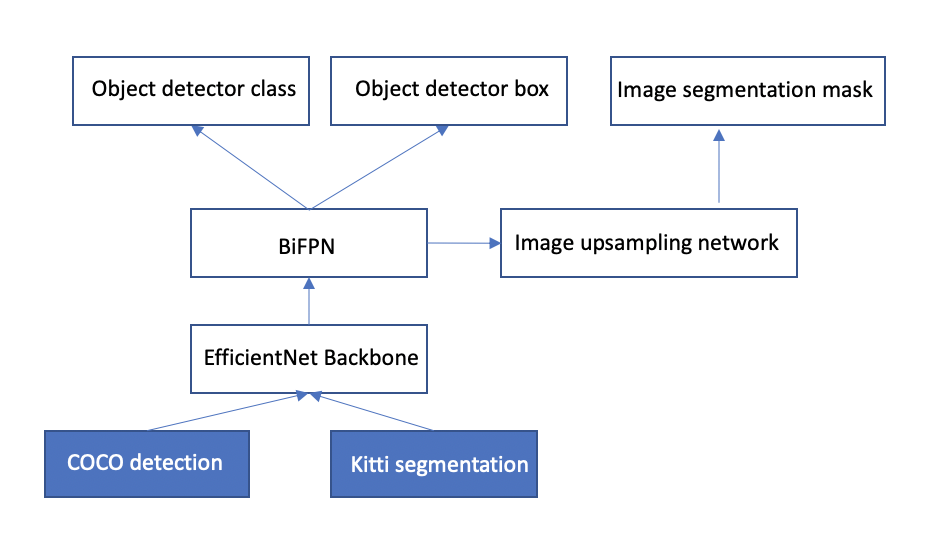
\includegraphics[width=0.8\textwidth]{imgs/efficientdet-multi.png}
    \caption{EfficientDet model with segmentation and detection heads.}
\end{figure}

With the segmentation head and object detector head configured, it would now be easy to extend this model further.
We could easily add a new image classification head using the same backbone, like \citep{multinet}, where a single model is used for road segmentation, car detection, and road type classification.
Adding more classes to the segmentation or to the object classifier would be relatively easy to do.
Of course, there is a lot of sharing optimization to be done as well.
In our implementation, we naively shared everything, which was likely relatively detrimental to performance.
It would make sense to at least have the BiFPN be task-specific.
And since everything is now configured in the same model, it would be relatively easy to chop half of the backbone for each task and possibly get better results.
As we have covered over and over again, the space for possible improvements is huge.

\section{Overview of the experiments}
Based on our experiments, we can say that multi-task learning is hard when compared to training single-task models.
Training multiple single-task models is easier and faster and requires less user input and parameter optimization.
The effect of many parameters, like the learning rate, can be evaluated relatively easily based on a few epochs in a single task setting.
Perhaps to find the very best model, more experimentation and exploration is needed, but just some default values can generally provide good results.

For someone with little experience in training multi-task models, it can be difficult to get started.
Whereas it is easy to find multiple examples of just how a training loop should be created, finding such examples for multi-task models is much more difficult.
For experimenting with different ways of splitting the features into local and global features, it is important to have systems for easily doing experiments on different architectures.
In our experiments, we created four points where it was possible to cut the last block in the ResNet, for example, so it was easy to create models that each had none to some local features.
Devising ways to split on a more fine-grained level and grouping tasks when there are multiple would be extremely important when searching for the optimal architecture.
Manually changing how the weights are shared would not be enough.
In our experiments, this was also quite clear, as we did not experiment beyond having models that have some or none local features.
We did not do any experiments where we would have grouped the features in a more well thought out way.
Likely, most benefits are gained when multiple tasks share half of the networks instead of only having a head be local.
This would make sense as the lower level features are more general and likely there would not be as many conflicts as in the deeper layers.
The number of things to tune is also quite discouraging when the model does not train properly.
Finding out which part of the modifications to the default process is wrong can be extremely difficult.
Some of the mistakes we encountered were difficult and frustrating to solve. 
For example, we forgot to do a deep copy of the local features and just passed the same features as references to all tasks and wondered why the training of a single task was impacting others so much.
Or when we froze all local features except the head when we meant only to freeze all the global features.
Or mixing up the order of the tasks in the model task heads, so the final inferences ended up being complete garbage.

The impact of the various parameters that have to be picked seemed to be much larger.
With an incorrect sampling ratio, the models could be extremely far from the good sampling ratios.
It seems that finding the perfect sampling ratio might not be possible, and settling for a good enough one might be a good idea.
It seems that it may be a good idea to pick a lower learning rate than normal to find the best intersection of features.

Finally, the model structure's changes to create the various classifiers' heads can be difficult to add.
While adding multiple image classifiers is relatively trivial to do if one is comfortable doing basic model definitions, it can be difficult to combine the various task heads for the more complex tasks.
For example, object detector models are generally provided with very specific training loops, so getting an object detector that has a classifier head is much more difficult than just training the two separately.
Without some easy way of abstracting the classifier heads and automatically injecting them into the training loop, it may not be possible for some to create multi-task models without extensive help.
We considered relatively simple tasks that already had open-source implementations and mostly combined them into a single model.
When dealing with some more advanced models like some of the ones presented in the multi-tasking chapter, it would be even more difficult to create the models.

Despite all the challenges, we did manage to create models that came close or were equal to their single-task counterparts.
The multi-task models were smaller and faster in those cases, confirming that using the shared representations can be an excellent idea.